\chapter{Matériel et pré-traitement des données }% construction des métriques
La biomasse de zooplancton et micronecton, l'assemblage des communautés phytoplanctoniques, l'environnement physique des organismes ne sont pas directement mesurables, ce sont des construits (\textit{constructs}), c'est à dire des abstractions qui décrivent le phénomène théorique d'intérêt \cite{edwards2000nature}. Pour étudier ces phénomènes, nous avons besoin de trouver des variables mesurables pouvant les décrire, c'est l'opérationnalisation du construit. Les choix des variables utilisées sont justifiées par la connaissances théorique des phénomènes étudiés, appuyés par la littérature. Les variables mesurables sont alors dites variables \textit{proxy} pour les construits associés. \cite{shmueli2010explain}.
 
 
 Les variables proxy sélectionnées sont les suivantes : (1) le Nautical Area Scattering Coefficient(NASC) approxime la biomasse du zooplancton et micronecton sur l'ensemble de la profondeur considérée; (2) les concentrations pigmentaires ($P_1, \ldots, P_9$) approximent l'assemblage des communautés phytoplanctoniques leur abondance totale; (3) le Finite-Time Lyapunov Exponent (FTLE) approxime l'hydrodynamisme et (4) la température et la salinité rendent compte des conditions physico-chimiques du milieu.
 
 Toutes les données utilisées pour cette étude sont des données secondaires, c'est-à-dire que le plan d'échantillonnage n'a pas été construit spécifiquement pour répondre à cette problématique.
 
 \section{Zone d'étude et plan d'échantillonnage}
 
 L'étude a été réalisée sur les années 2018, 2021, 2022 et 2023, en saison estivale (janvier-mars) afin de limiter la variabilité saisonnière, et de jour (calculé selon l'angle solaire), afin de limiter l'effet de la migration verticale journalière (DVM) \footnote{Déplacement synchronisé dans la colonne d'eau au rythme du cycle jour/nuit : les organismes résident en profondeur durant le jour et remontent vers la surface la nuit, principalement pour se nourrir tout en réduisant le risque de prédation visuelle en eaux éclairées. Ce phénomène est considéré comme le plus grand mouvement synchronisé de biomasse à l'échelle de la planète. \cite{Bandara2021}}. La fenêtre d'étude a été fixée à [45,90]°E de longitude et [30, 60]°S de latitude afin de cibler précisémment le secteur indien de l'Océan Austral.
 
 \section{Données d'acoustique active (OBSAUSTRAL) et construction du Nautical Area Scattering Coefficient (NASC)}
 
 \subsection{Données d'acoustique active}
 Les données d'acoustiques actives ont été collectées par transects \footnote{Le bateau se déplace et collecte en même temps des données, par opposition aux données "stations" collectées lorsque le bateau est en arrêt. Cela a un coût en terme de résolution des spectrogramme et d'interprétabilité mais permet d'obtenir une plus grande couverture spatiale.} lors des campagnes océanographiques OBSAUSTRAL/THEMISTO 2018, 2021, 2022, 2023 en saison estivale. Ils sont détaillés sur la figure \ref{fig:transectsparannee2} \cite{flotteoceanographique_campagnes}.  
 \begin{figure}[H]
 	\centering
 	\includegraphics[width=0.6\textwidth]{images/02\_materiel\_et\_methode/active\_acoustic\_et\_NASC/transects\_par\_annee\_2}
 	\caption{Carte des transects effectués par le Marion Dufresnes II lors des campagnes océanographiques OBSAUSTRAL/THEMISTO 2018, 2021, 2022 et 2023.}
 	\label{fig:transectsparannee2}
 \end{figure}
 
 \vspace{1cm}
 
 Deux fréquences d'émissions ont été sélectionnées: 38 kHz, afin de comparer nos résultats avec la littérature \footnote{La méthode d'acoustique active ayant été développée par les pêcheries, la fréquence d'échosondeur de référence est 38kHz (fréquence à laquelle les poissons sont facilement détectables).} et 120 kHz, fréquence à laquelle les zooplanctons d’intérêts, Euphausiacés (krill) et Copépodes, sont les plus détectables (voir Annexe \ref{annexe:rep_freq}, figure \ref{fig:freqresponse}). Les échogrammes (figures \ref{fig:echogramme38khz2023-01-28} et \ref{fig:echogramme120khz2023-01-28}) donnent un aperçu de la nature des données collectées et de la manière dont l'information contenue par le signal reçu (résolution, organismes visibles) est déterminée par la fréquence de l'onde émise. Une forte intensité de l’écho reçu traduis la présence d'une importante biomasse d'organisme à ce temps, localisation géographique et profondeur.
 
 \begin{figure}[H]
 	\centering
 	\begin{subfigure}[t]{0.7\textwidth}
 		\centering
 		\includegraphics[width=\textwidth]{images/02\_materiel\_et\_methode/active\_acoustic\_et\_NASC/echogramme\_38kHz\_2023-01-28.png}
 		\caption{Fréquence d'émission de 38 kHz}
 		\label{fig:echogramme38khz2023-01-28}
 	\end{subfigure}
 	\vfill
 	\begin{subfigure}[t]{0.7\textwidth}
 		\centering
 		\includegraphics[width=\textwidth]{images/02\_materiel\_et\_methode/active\_acoustic\_et\_NASC/echogramme\_120kHz\_2023-01-28.png}
 		\caption{Fréquence d'émission de 120 kHz}
 		\label{fig:echogramme120khz2023-01-28}
 	\end{subfigure}
 	\caption{Exemple d'échogramme obtenu le 2023-01-28 entre 18h et 00h aux fréquences (a) 38 kHz et (b) 120 kHz}
 	\label{fig:echogramme2023-01-28}
 \end{figure}
 
 \subsection{Construction du Nautical Area Scattering Coefficient (NASC)}
 
	 L'\textbf{Intensité de l'echo (Echo Level EL) }correspond au signal reçu par le transducteur lorsqu'une onde est émise dans la colonne d'eau puis réfléchis par un objet.
	 \begin{equation}
	 	EL = SL - 2TL + DI + TS
	 \end{equation}	
	 où 
	 \begin{itemize}
	 	\item SL (Source Level): intensité du son émise (dB) $SL = 10 \times \log_{10}(I/I_{ref}) $ et $I_{ref} = \rho_{ref}^{2} = 1 \mu \text{Pa}$ ($\rho_{ref}$ la pression de référence)
	 	\item TL (Transmission Loss): perte de transmission  \footnote{Le premier terme correspond à l'attenuation due à la dispersion de l'onde et le second terme correspondant à l'éttenuation de la propagation du milieu ($\alpha$ le coefficient d'absorption en $dB.m^{-1}$)} $TL = 20 \log_{10} (R) + \alpha R$
	 	\item DI (Directivity Index): indice de directivité du transducteur (dB)
	 	\item TS (Target Strength): réfléctivité de la cible 
	 \end{itemize}
	 
	 \vspace{0.5cm}
	 
	 La \textbf{section efficace de rétrodiffusion} \(\sigma_{bs} = 10^{\frac{TS}{10}}\)  (\(\mathrm{m^2}\)) caractérise la capacité de la cible à rétrodiffuser l'énergie acoustique. 
	 %et est déterminée par référence à la section efficace de rétrodiffusion théorique de la sphère de calibration utilisée lors de la calibration du sondeur. 
	 
	 \vspace{0.5cm}
	 
	 Le \textbf{volume backscattering coefficient} $s_v$ (en $m^{2}.m^{-3}$ ou $m^{-1}$) est la somme  toutes les surfaces réfléctives $\sigma_{bs}$ de toutes les cibles acoustiques dans le volume d'échantillonage $V_0$, normalisées à 1$m^{3}$.  
	 \begin{equation}
	 	s_v = \sum \sigma_{bs}/V
	 \end{equation}
	 Il mesure la densité acoustique des organismes présents dans un volume d'eau. Un niveau de $s_v$ élevé correspond à une quantité plus importante de rétrodiffusion acoustique dans le volume échantillonné. Ce qui est interprété comme un nombre important d'organismes présents dans la colonne d'eau ou un organisme de taille importante ou encore un organisme ayant des propriétés fortement rétrodiffusantes \footnote{De nombreux poissons pélagiques présentent des vessies natatoires gazeuses ou lipidiques, organes leurs permettant d'ajuster leur flottabilité. A 38 kHz, ces organes ont des propriétés retro-diffusantes particulières : ils amplifient le signal}. Par convention, on exprime souvent cette grandeur en échelle logarithmique sous le nom de Volume Backscattering Strength, noté $S_v \text{ (dB re 1 m}^{-1})$ tel que $s_v = 10^{\frac {S_v} {10}}$.
	 
	 \vspace{0.5cm}
	 
	 Le \textbf{Nautical Area Scattering Coefficient (NASC)}, noté $s_A$, correspond au coefficient de rétrodiffusion acoustique par unité de surface nautique (en $m^{2}.nmi^{-2}$). Il résume la rétrodiffusion acoustique sur une couche d'eau donnée en intégrant entre deux profondeurs le volume backscattering coefficient $s_v$ multiplié par un certain facteur (convention) :
	 \begin{equation}
	 	s_A = 4 \pi (1852)^{2} \int_{z_{1}}^{z_{2}} s_v(z) dz
	 \end{equation}
	 
	 Dans le cadre de cette étude, la profondeur d'intégration $z_1$ a été fixé à 25 m pour limiter le bruit d’échantillonnage de surface \footnote{effet de "bullage" du bateau bruitant les données à des faibles profondeurs}. Le choix de $z_2$ dépend de la fréquence de l'échosondeur : pour des fréquences de 38 kHz et 120 kHz, la colonne d'eau est échantillonné respectivement jusqu'à une profondeur moyenne de 700 m et 300 m. En effet, à partir de ces profondeurs, beaucoup de données $s_v$  sont manquantes (voir Annexe \ref{annexe:missing_values}, figure \ref{fig:diagnabydepthperesu}). Les profils avec plus de 50\% de valeurs manquantes ont été exclus du jeu de données. Les valeurs manquantes résiduelles ont été comblées : (1) par interpolation linéaire lorsque situées entre deux valeurs connues et (2) par prolongation de la valeur la plus proche, lorsque situées aux extrémités. 
	 
	 \vspace{0.5cm}
	 
	 Ainsi, pour chaque profil de $S_v$, on calcule le NASC et obtenons un scalaire, qui résume le volume de rétrodiffusion acoustique sur l'ensemble de la couche d'eau considérée ([25-700]m pour 38kHz et [25-300]m pour 120kHz). La figure \ref{fig:nasc} présente le NASC en fonction du temps pour le transect 2023 OBSAUSRAL.
 
	\begin{figure}[H]
		\centering
		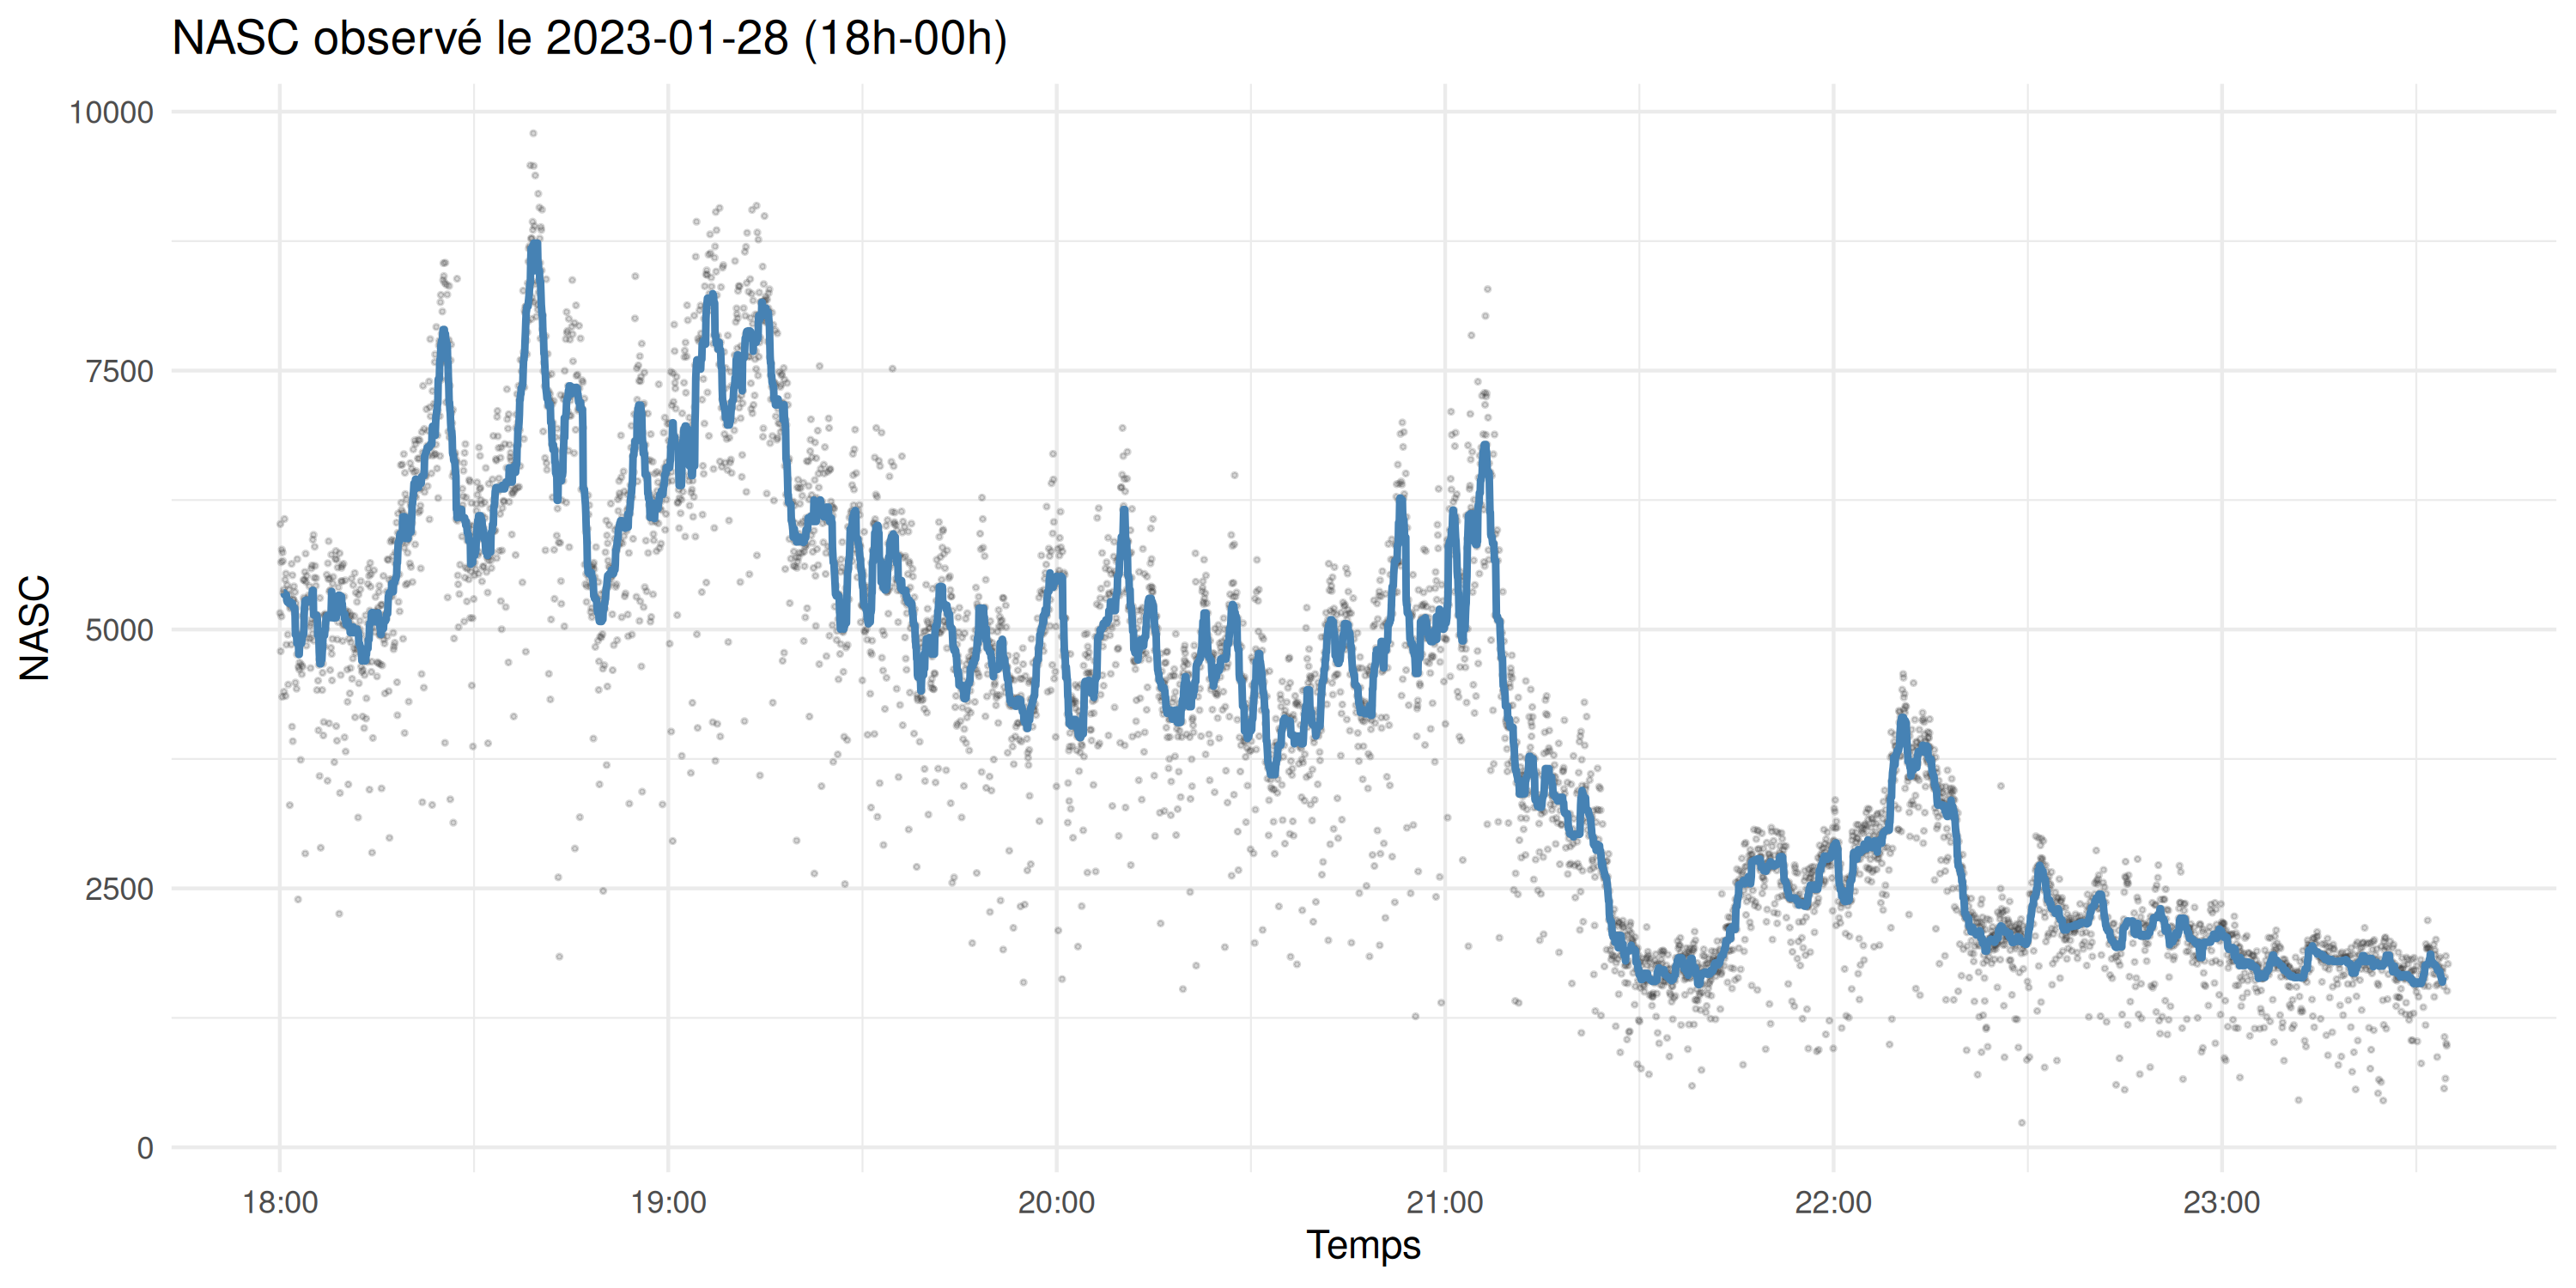
\includegraphics[width=0.7\textwidth]{images/02_materiel_et_methode/active_acoustic_et_NASC/nasc_2023-01-28_smooth_bis}
		\caption{NASC en fonction du temps le 2023-01-28, données d'acoustique active (transect) issues de la campagne océanographique OBSAUSTRAL 2023 \cite{flotteoceanographique_campagnes}.}
		\label{fig:nasc}
	\end{figure}
	 
 
 
 
 
 
 
 
 
 \section{Concentrations de pigments photosynthétiques (PIGMeANN)}
	 La couleur des océans dépend de leur composition en pigments et ces pigments sont contenus dans les organismes phytoplanctoniques. L'analyse de la couleur des océans à partir d'images satellite permet donc d'étudier les communautés phytoplanctoniques sur une échelle spatiale et temporelle large. L'algorithme PIGMeANN \cite{sari2026regional} associe, à l'aide de réseaux neuronaux profonds, une empreinte spectrale \footnote{Forme caractéristique du spectre de la lumière réfléchie par l'eau, c'est-à-dire de la façon dont la réflectance varie selon la longueur d'onde. Chaque pigment absorbe la lumière à des longueurs d'onde précises : des communautés de composition pigmentaire différente produisent donc des spectres de forme différente.} à des mesures de concentrations de pigments phytoplanctoniques \textit{in-situ} obtenues par High Performance Liquid Chromatography (HPLC) \footnote{Permet de séparer et quantifier les pigments afin d’identifier les différents groupes phytoplanctoniques présents. L’échantillon est injecté dans une colonne traversée par un solvant sous haute pression, où ses différents composés sont séparés puis détectés individuellement.}. Ainsi, cette méthode permet de prédire les concentrations de neuf pigments phytoplanctoniques sur l'ensemble de la ROI. Ils sont détaillés dans le tableau \ref{tab:pigments}.
	
	\begin{table}[H]
		\centering
		\footnotesize
		\setlength{\tabcolsep}{3pt}
		\renewcommand{\arraystretch}{1.3}
		\begin{tabularx}{\textwidth}{
				>{\raggedright\arraybackslash}p{1.3cm}
				*{9}{>{\centering\arraybackslash}X}
			}
			\hline
			\textbf{Pigment} & Divinyl chloro\-phylle $a$ & Chloro\-phylle $a$ & Chloro\-phylle $b$ & Zéaxan\-thine & Fucoxan\-thine & 19'-hexanoyl\-oxyfuco\-xanthine & 19'-butanoyl\-oxyfuco\-xanthine & Allo\-xanthine & Péri\-dinine \\
			\hline
		\end{tabularx}
		\renewcommand{\arraystretch}{1}
		\caption{Neuf pigments photosynthétiques dont les concentrations sont estimées par l'algorithme PIGMeANN \cite{sari2026regional}.}
		\label{tab:pigments}
	\end{table}
	
	La figure  \ref{fig:mapchla2023-01-26} illustre la prédiction par PIGMeANN de la Chorophylle-a le 2023-01-26 sur le secteur étudié. Les zones non colorées correspondent sont des données manquantes. La forte couverture nuageuse de la région induit une absence de données satellitaires, et donc des concentrations prédites par PIGMeANN.
	 
	\begin{figure}[H]
		\centering
		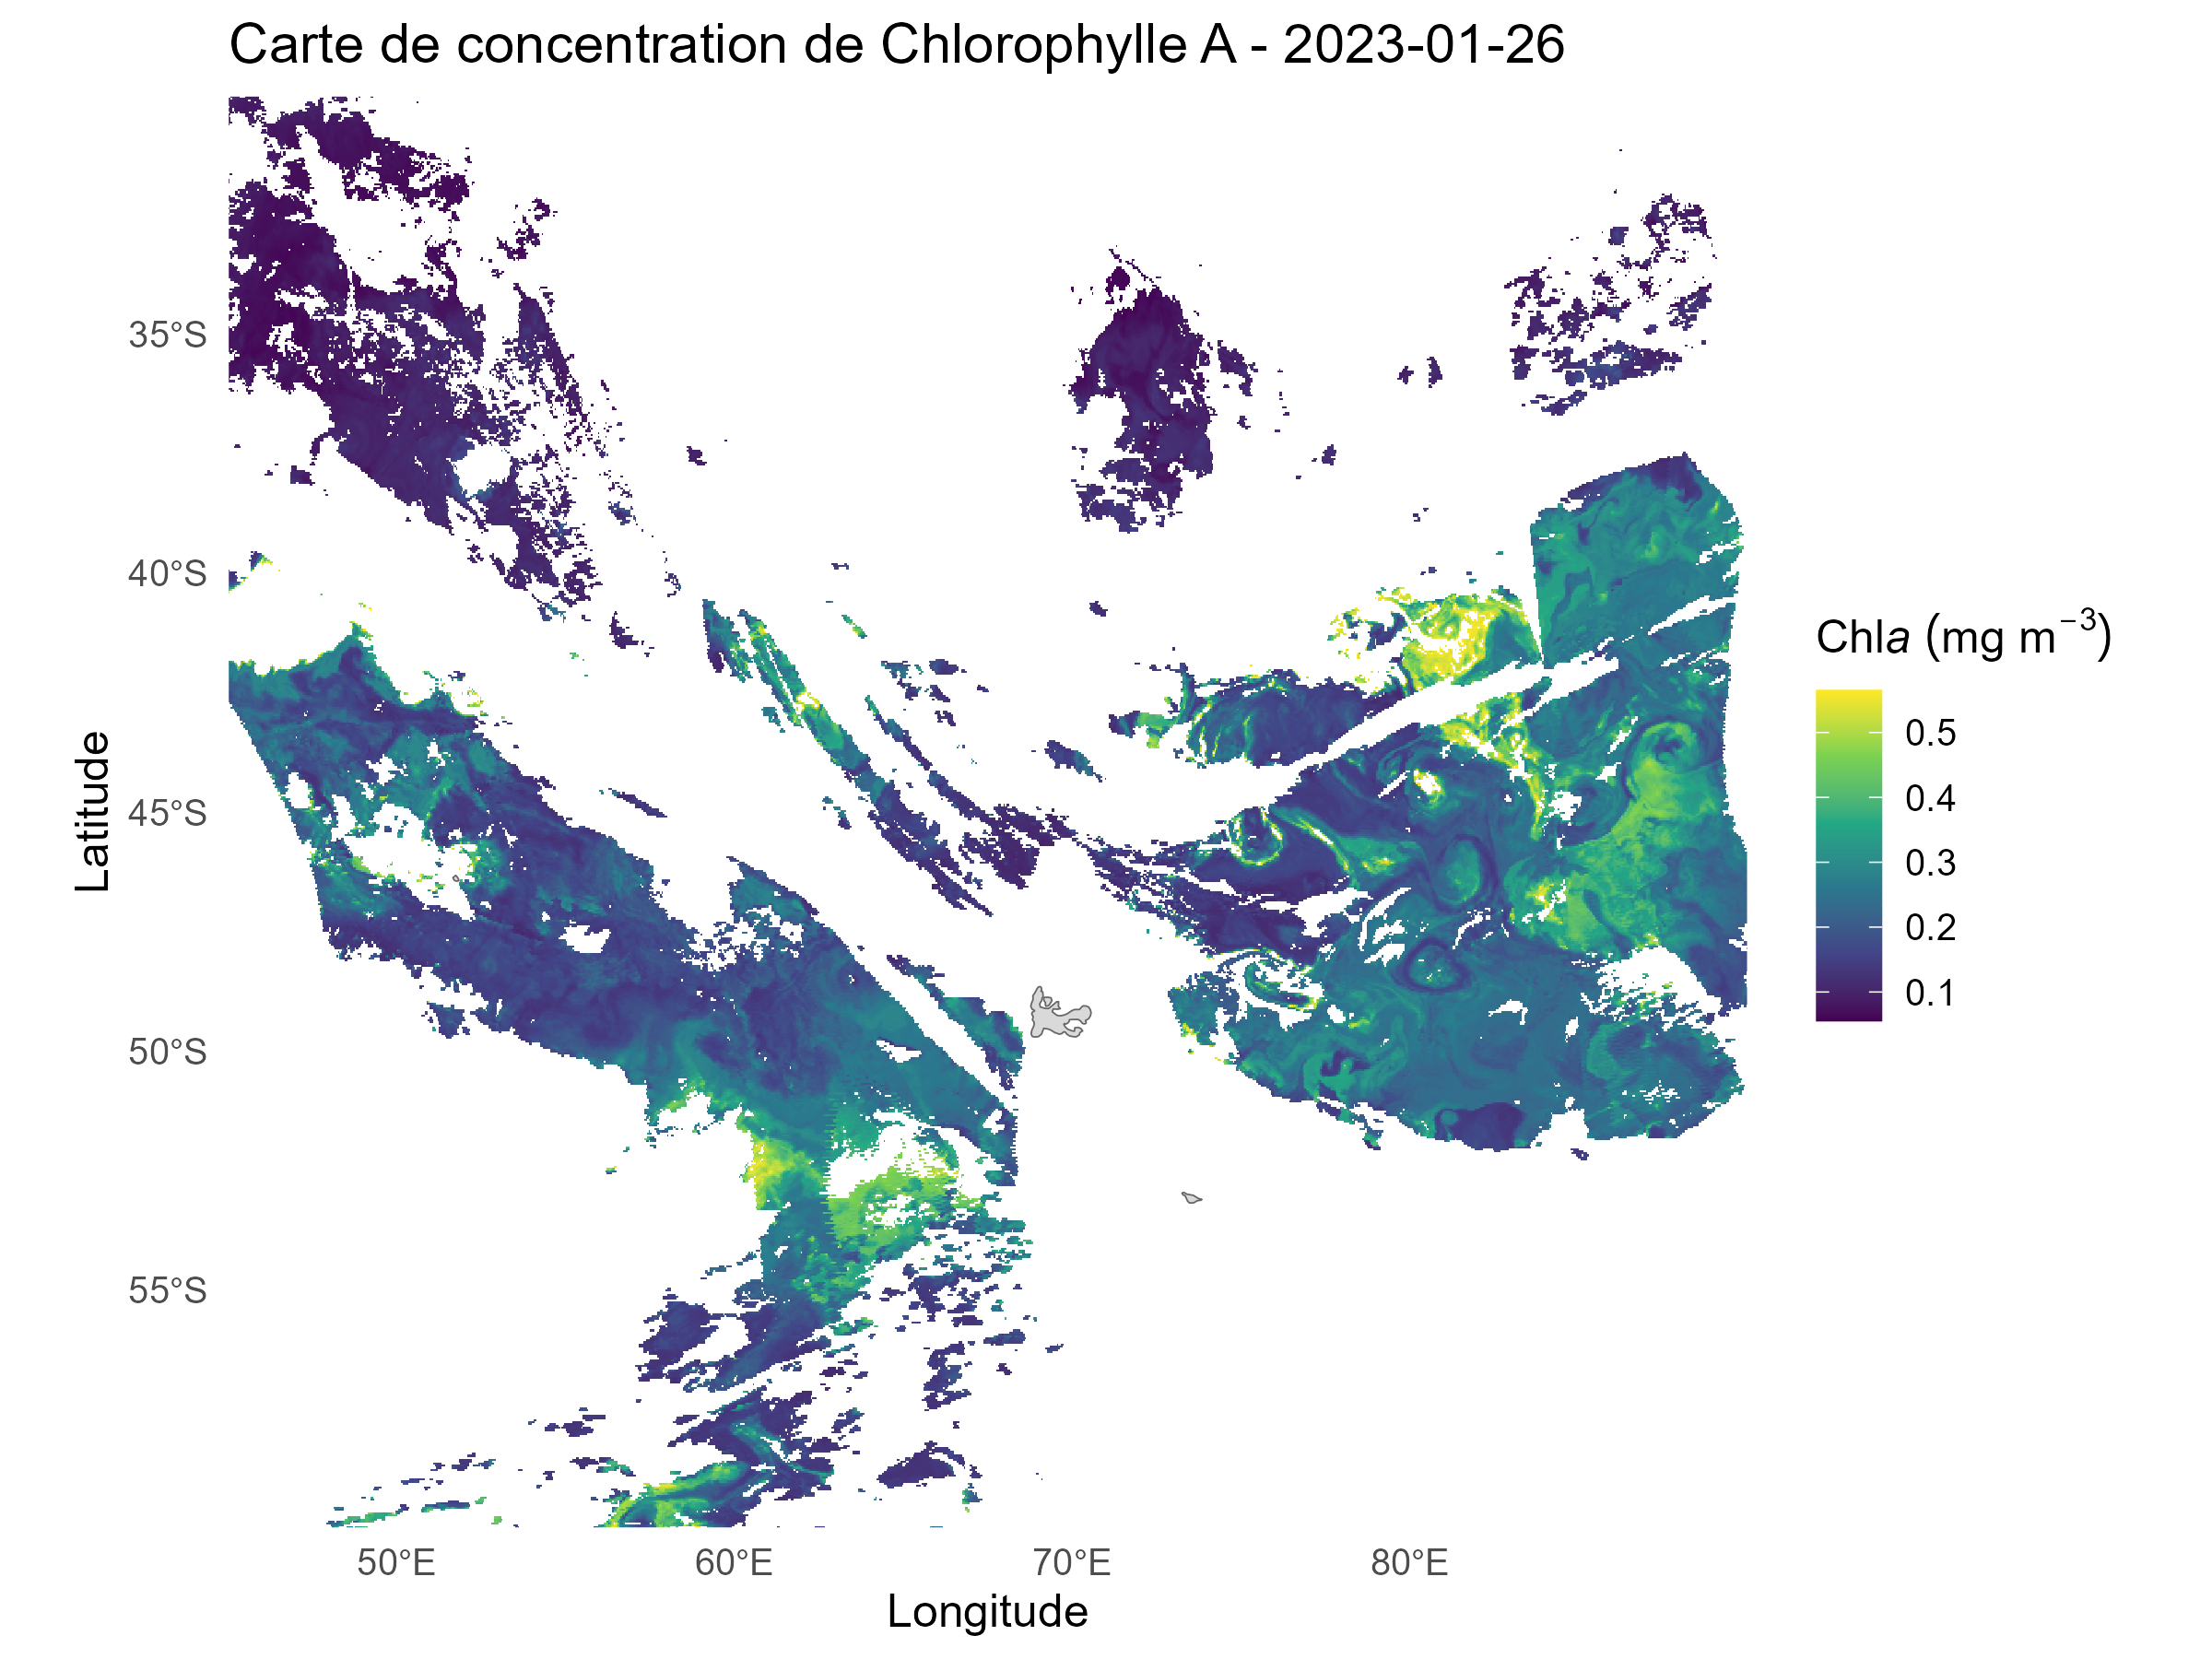
\includegraphics[width=0.7\textwidth]{images/02_materiel_et_methode/map_chla_2023-01-26}
		\caption{Carte de prédiction de la concentration de Chlorophylle-a le 2023-01-26 sur le secteur indient du SO, prédictions issue de l'alorithme PIGMeANN développé par Sari el Dine \cite{sari2026regional}. La présence de nuages gène grandement la prédiction sur la zone totale.}
		\label{fig:mapchla2023-01-26}
	\end{figure}
	 
	Plutôt que les concentrations pigmentaires absolues, on s'intéresse aux concentrations relative, c'est-à-dire le ratio des concentrations de pigments sur la somme des concentrations pigmentaires totale (Chlorophylle-a exclue \footnote{ubiquitaire, elle n'apporte pas d'information sur la composition de la communauté}) :
	 
	 \begin{equation}
	 	R_i = \frac{[\text{Pigment}_i]}{\displaystyle\sum_{j \neq \text{Chla}} [\text{Pigment}_j]}
	 	\label{eq:ratio_pigment}
	 \end{equation}
	 
	 La concentration relative $R_i$ la plus importante à une certaine localisation et temps permet d'identifier hypothétiquement les classes taxonomique (Phytoplanctonique Functional Types, PFT) ou de taille (Phytoplanctonic Size Class, PSC)  dominantes de la communauté, par association avec les connaissances théoriques développées dans la littérature \cite{sari2025influence}, \cite{heidemann2024drivers} \cite{Georges2014}. Ces correspondances sont détaillées dans le tableau \ref{tab:corresp_pig}. L'abondance totale de phytoplancton est estimée par la concentration absolue en Chlorophylle-a, pigment ubiquitaire présent chez la majorité des organismes photosynthétiques.
	 % J'hésite à mettre ça en Discussion
 
 	\begin{table}[H]
 		\centering
 		\renewcommand{\arraystretch}{1.3}
 		\begin{tabular}{
 				>{\raggedright\arraybackslash}p{3.4cm}
 				>{\raggedright\arraybackslash}p{2.0cm}
 				>{\raggedright\arraybackslash}p{4.8cm}
 				>{\raggedright\arraybackslash}p{2.6cm}
 			}
 			\hline
 			\textbf{Pigment} & \textbf{Abréviation} & \textbf{Groupe phytoplanctonique associé (PFD)} & \textbf{Classe de taille (PSC)} \\
 			\hline
 			Divinyl chlorophylle $a$ & dvChla & Procaryotes picoplanctoniques (\textit{Prochlorococcus}) & Picophytoplancton \\
 			Chlorophylle $a$ & Chla & Marqueur de biomasse totale (tous groupes) & -- \\
 			Chlorophylle $b$ & Chlb & Chlorophycées / Prasinophycées & Picophytoplancton \\
 			Zéaxanthine & Zea & Cyanobactéries (\textit{Synechococcus}) & Picophytoplancton \\
 			Fucoxanthine & Fuco & Diatomées (dominantes) & Microphytoplancton \\
 			19'-hexanoyloxyfucoxanthine & Hex & Prymnésiophycées (haptophytes) & Nanophytoplancton \\
 			19'-butanoyloxyfucoxanthine & But & Prymnésiophycées / pélagophytes & Nanophytoplancton \\
 			Alloxanthine & Allo & Cryptophycées & Nanophytoplancton \\
 			Péridinine & Per & Dinoflagellés (péridiniens) & Microphytoplancton \\
 			\hline
 		\end{tabular}
 		\renewcommand{\arraystretch}{1}
 		\caption{Pigments photosynthétiques analysés et groupes phytoplanctoniques hypothétiquement associés (PFD et PSC) dans le secteur de Kerguelen en été austral, d'après \cite{Lasbleiz2014}, \cite{sari2025influence}}
 		\label{tab:corresp_pig}
 	\end{table}
 
 \section{Données modèles de température et salinité (CMEMS) et calcul des Domaines Océanographiques Fonctionnels (FOD)}
	 \subsection{Données modèles de température et salinité (CMEMS)}
		\label{section:temp_sal}
		 Les données de températures et salinité font partie du jeu de données "Global Ocean Physics Reanalysis" (la réanalyse GLORYS12V1, GLOBAL\_MULTIYEAR\_PHY\_001\_030) \cite{cmems_glorys12}, issues de la plateforme Copernicus \footnote{Programme d’observation de la Terre de l’Union européenne, qui fournit notamment des données et services permettant de surveiller et comprendre l’état de l’environnement, dont l’océan \cite{copernicus2026services}}. Ce sont des données issues des observations temps-réelles CMEMS \footnote{Copernicus Marine Environment Monitoring Service, service marin de Copernicus} et réanalysées par le modèle NEMO \footnote{Nucleus for European Modelling of the Ocean, modèle numérique de l’océan qui simule l’évolution de paramètres comme la température, la salinité, les courants et le niveau de la mer}, et ERA5 \footnote{Modèle atmosphérique de l'ECMWF (European Centre for Medium-Range Weather Forecasts) qui fournit les conditions atmosphériques nécessaires pour forcer le modèle océanique NEMO à sa surface}. Elles ont une résolution spatiale de 0.083° et une résolution temporelle journalière.
		 Afin d'alléger le traitement des données, seules les mesures de température et de salinité comprises entre 20 et 500 m de profondeur ont été conservées. La figure \ref{fig:T_S_profile} présente un exemple de profile de température et salinité à 50°E de longitude, 60°S de latitude, le 2023-01-26.
		\begin{figure}[H]
			\centering
			\includegraphics[width=\linewidth]{images/02\_materiel\_et\_methode/TS\_FOD/profils\_TS\_2023-01-26.png}
			\caption{Profil de Température et de Salinité issue de GLORYS (CMEMS), tronqués en deçà de 20m et au delà de 500m aux coordonnés (50°E, 60°S).}
			\label{fig:T_S_profile}
		\end{figure}
 
 	\subsection{Calcul des Domaines Océanographiques Fonctionnels (FOD)}
	 	Les Domaines Océanographiques Fonctionels (FOD, Functional Oceanographic Domain) sont des masses d'eau ayant des caractéristiques thermohalines similaires. La méthode d'identification des FOD a été développée par Fonvieille N. et Nerini D. \cite{fonvieille2024}. Les profils de température et salinité sont, dans un premier temps (1), estimées dans un espace fonctionnel par projection sur une base de B-spline. Dans un second temps (2), la dimension de la matrice des coefficients de pondération des B-splines est réduite par Analyse par Composante Principale (PCA, Principal Componant Analysis). Dans un dernier temps (3), un clustering (GMM) est appliqué à $K$ composantes principales déterminé par la PCA de l'étape précédente. Ces trois étapes sont développées en Annexe \ref{annexe:methode_fod}.
	 	
	 	\vspace{0.3cm}
	 	
	 	Dans notre étude, l'estimation par projection sur une base de B-splines a été effectué avec l'hyperparamètre de régularisation $\lambda = 0.25$, pour $K=25$ B-splines. Sont conservées pour le clustering 6 composantes principales ($>0.99$ \% explained var., voir tableau \ref{tab:pca_variance}). L'indice BIC nous permet de sélectionner $nclust = 6$ clusters. En ajoutant les classes de transitions (les soft classes, c'est-à-dire toutes les données dont la probabilité d'appartenance au cluster le plus probable est inférieure à $thr  = 0.75$), on obtient alors 13 clusters distincts (7 clusters de "transitions") \footnote{La classe "NA" correspond aux clusters manquants sur le plateau de Kerguelen. Les profils de température et salinité allant de 20 à 500m, sont retirés des calculs tout profils ayant des données manquantes entre ces deux valeurs. Les zones où la bathymétrie est inférieure à 500m sont donc exclues de ces calculs.}, ce sont les 13 Domaines Océanographiques Fonctionnels (FOD).
	 	
		\begin{figure}[H]
			\centering
			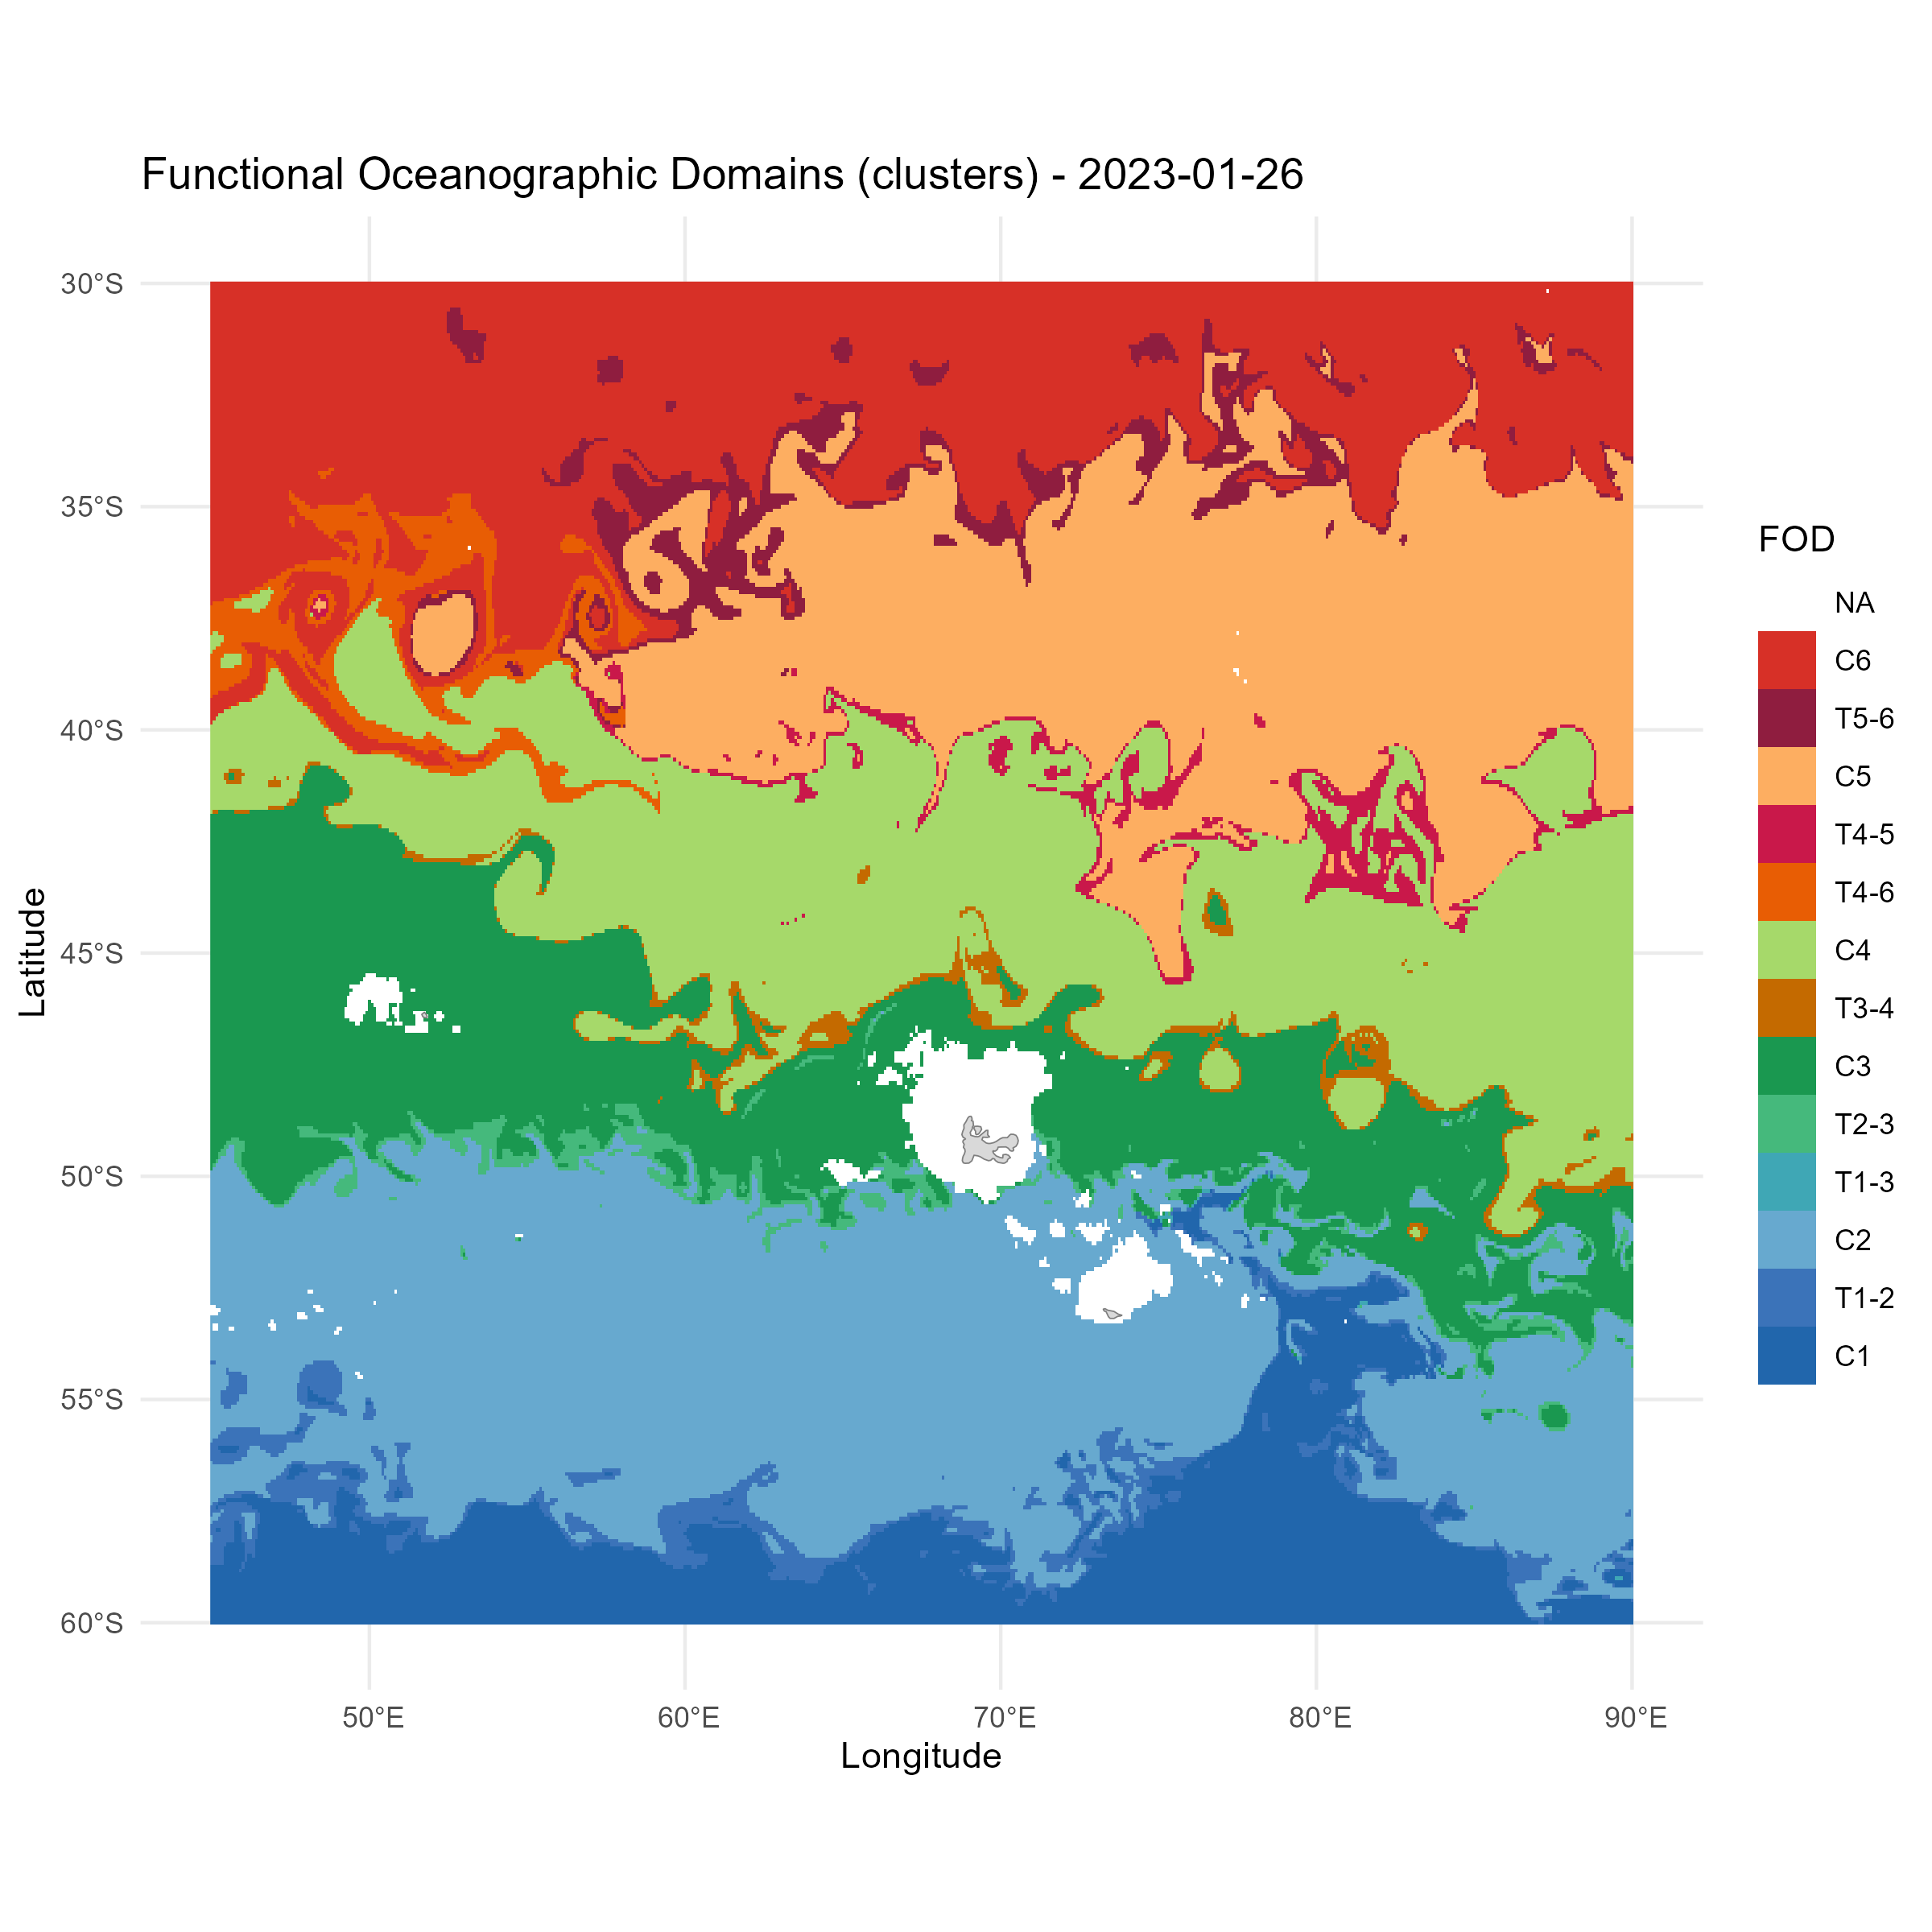
\includegraphics[width=0.8\textwidth]{images/02_materiel_et_methode/TS_FOD/cluster_transition_map_renamed_20230126}
			\caption{Carte des Domaines Océanographiques Fonctionnels du 2023-01-26 générée par la méthode développée par Fonvieille N. et Nerini D. \cite{fonvieille2024}.}
			\label{fig:fodmap}
		\end{figure}
		
	 	\begin{figure}[H]
	 		\centering
	 		\begin{subfigure}[b]{0.48\textwidth}
	 			\centering
	 			\includegraphics[width=0.7\textwidth]{images/02\_materiel\_et\_methode/TS\_FOD/temperature\_clusters\_transitions.png}
	 			\caption{Profil de température (°C) moyen par cluster}
	 		\end{subfigure}
	 		\hfill
	 		\begin{subfigure}[b]{0.48\textwidth}
	 			\centering
	 			\includegraphics[width=0.7\textwidth]{images/02\_materiel\_et\_methode/TS\_FOD/salinity\_clusters\_transitions.png}
	 			\caption{Profil de salinité (PSU) moyen par cluster}
	 		\end{subfigure}
	 		\caption{}
	 		\label{fig:temp_sal_cluster}
	 	\end{figure}
	 	
	 	 La figure \ref{fig:fodmap} illustre les 13 FOD capturés le 2023-01-26. Pour chacun des FOD, les profils de température et de salinité moyennés sur l'ensemble de la période d'étude sont présentés en figure \ref{temp_sal_cluster}. Chaque FOD correspond donc une masse d'eau ayant des propriétés thermohalines similaires. La projection de ces FOD sur une carte permet également de visualiser l'hydrodynamisme de la région. Les fronts sont des zones de rencontres entre des masses d'eau ayant propriétés hydologiques différentes. Les FOD de "transition" permettent de les identifier : T2-3 correspond à la transition entre le cluster 2 et le cluster 3. Sa latitude ($\approx 50$°S) permet de l'identifier comme Front Polaire. En suivant la même méthode, on peut identifier le Front Subantarctique (T3-4) et le front sub-tropical (T4-5/T4-6). Les tourbillons sont des courants en vortex, ce qui empêche les masses d'eau de se mélanger entre elles. Ainsi, on peut également identifier les tourbillons sur les cartes de FOD : ce sont les régions où, localement, un FOD est présent, entouré par un autre FOD dominant. Sur la figure \ref{fig:fodmap}, on remarque par exemple un tourbillon aux coordonnées (53°E, 27°S) environ : le cluster 5 est pris dans un tourbillon.
 	
 \section{Champs de courants modèles (CMEMS) et calcul du Finite Time Lyapunov Exponent (FTLE)}
 \subsection{Données de Champs de courants modèles (CMEMS)}
 	Les champs de courants sont des données modèles également issues du modèle de réanalyse océanique GLORYS12 du Copernicus Marine Service (CMEMS), détaillé en section \ref{section:temp_sal}. Les champs de courants de surface (composantes zonale (u) et méridienne (v)) en sont extraits avec une résolution journalière.  
 	
 \subsection{Calcul du Finite-Time Lyapunov Exponent}
	 Le Finite Time Lyapunov Exponent est un indicateur qui permet de caractériser la séparation ou la convergence de trajectoires de particules d’eau sur une durée finie. On peut ainsi identifier les structures dynamiques susceptibles de contrôler le transport et la dispersion dans l’océan \cite{shadden2005definition}, \cite{dovidio2004mixing}. Son calcul, effectué dans cette étude par Molinet M. \footnote{Doctorant au MIO et CEBC, encadrant de ce stage} est le suivant :
	 
	 On considère le champ de vitesse bidimensionnel dépendant de la position et du temps, issu des données de réanalyse GLORYS21 :
	 \begin{equation}
	 	\mathbf{u}(x,y,t)
	 	=
	 	\begin{pmatrix}
	 		u(x,y,t)\\
	 		v(x,y,t)
	 	\end{pmatrix}
	 \end{equation}
	 avec $u$ et $v$ représentant respectivement les composantes zonale et méridienne de la vitesse, et où $\mathbf{x}=(x,y)$ désigne la position de la particule.
	 
	 À partir d'une position initiale $\mathbf{x}_0$ au temps $t_0$, la trajectoire d'une particule est obtenue en intégrant, dans notre cas avec la méthode Runge-kutta (RK4), l'équation d'advection :
	 
	 \begin{equation}
	 	\frac{d\mathbf{x}}{dt}
	 	=
	 	\mathbf{u}(\mathbf{x},t),
	 	\qquad
	 	\mathbf{x}(t_0)=\mathbf{x}_0.
	 \end{equation}
	 
	 Après une durée d'intégration $T$, la position finale de la particule peut être décrite à l'aide du flot lagrangien :
	 
	 \begin{equation}
	 	\mathbf{x}(t_0+T)
	 	=
	 	\mathbf{F}_{t_0}^{T}(\mathbf{x}_0),
	 \end{equation}
	 
	 où $\mathbf{F}_{t_0}^{T}$ est l'application qui associe à chaque position initiale $\mathbf{x}_0$ sa position après une durée $T$.
	 
	 On peut ensuite analyser la variation des trajectoires $\mathbf{F}_{t_0}^T(x_0)$ après un temps $T$ si l'on change la position initiale $x_0$ des particules (tenseur de déformation): 
	 \begin{equation}
	 	\nabla \mathbf{F}_{t_0}^{T}
	 	=
	 	\frac{\partial \mathbf{F}_{t_0}^{T}}{\partial \mathbf{x}_0}
	 	=
	 	\begin{pmatrix}
	 		\frac{\partial F_x}{\partial x_0} &
	 		\frac{\partial F_x}{\partial y_0} \\[6pt]
	 		\frac{\partial F_y}{\partial x_0} &
	 		\frac{\partial F_y}{\partial y_0}
	 	\end{pmatrix}
	 \end{equation}
	 
	 Le tenseur de Cauchy-Green permet de quantifier la déformation des distances entre des particules initialement proches. Il est défini par :
	 \begin{equation}
	 	\mathbf{C}_{t_0}^{T}(\mathbf{x}0)
	 	=
	 	\left(
	 	\nabla\mathbf{F}{t_0}^{T}(\mathbf{x}0)
	 	\right)^{T}
	 	\nabla\mathbf{F}{t_0}^{T}(\mathbf{x}_0).
	 \end{equation}
	 
	 Le facteur maximal d'étirement entre les particules est donné par la plus grande valeur popre $\lambda_{max}$ du tenseur de Cauchy-Green $\mathbf{C}_{t_0}^{T} (\mathbf{x}_0)$
	 
	 Le FTLE ($\sigma_{t_0}^{T}$) est ensuite calculé, il correspond au taux de croissance logarithmique du facteur d'étirement maximal $\lambda_{max}$, normalisé par la durée d'intégration $T$ :
	 
	 \begin{equation}
	 	\sigma_{t_0}^{T}(\mathbf{x}_0)
	 	=
	 	\frac{1}{|T|}
	 	\ln\left(
	 	\sqrt{
	 		\lambda_{\max}\left(
	 		\mathbf{C}_{t_0}^{T}(\mathbf{x}_0)
	 		\right)
	 	}
	 	\right)
	 \end{equation}
	 
	 avec :
	 \begin{itemize}
	 	\item $\mathbf{C}_{t_0}^{T}$ le tenseur de Cauchy-Green, décrit comment les distances entre les particules évoluent. Il est calculé à partir des données de champs de courants
	 	\begin{equation}
	 		\mathbf{C}_{t_0}^{T}
	 		=
	 		\left(\nabla\mathbf{F}_{t_0}^{T}\right)^{T}
	 		\left(\nabla\mathbf{F}_{t_0}^{T}\right)
	 	\end{equation}
	 	\item $	\lambda_{\max}$ la plus grande valeur propre du tenseur de Cauchy-Green
	 	\item $\mathbf{x}_0$ la position initiale de la particule
	 	\item $T$ le tempsd d'intégration pendant lequel on suit la particule
	 	\item $\sigma$ le FTLE qui mesure le taux moyen de séparation des trajectoires des particules, exprimé en unité inverse du temps
	 \end{itemize}
	 
	 \vspace{0.5em}
	 
	\begin{figure}[H]
		\centering
		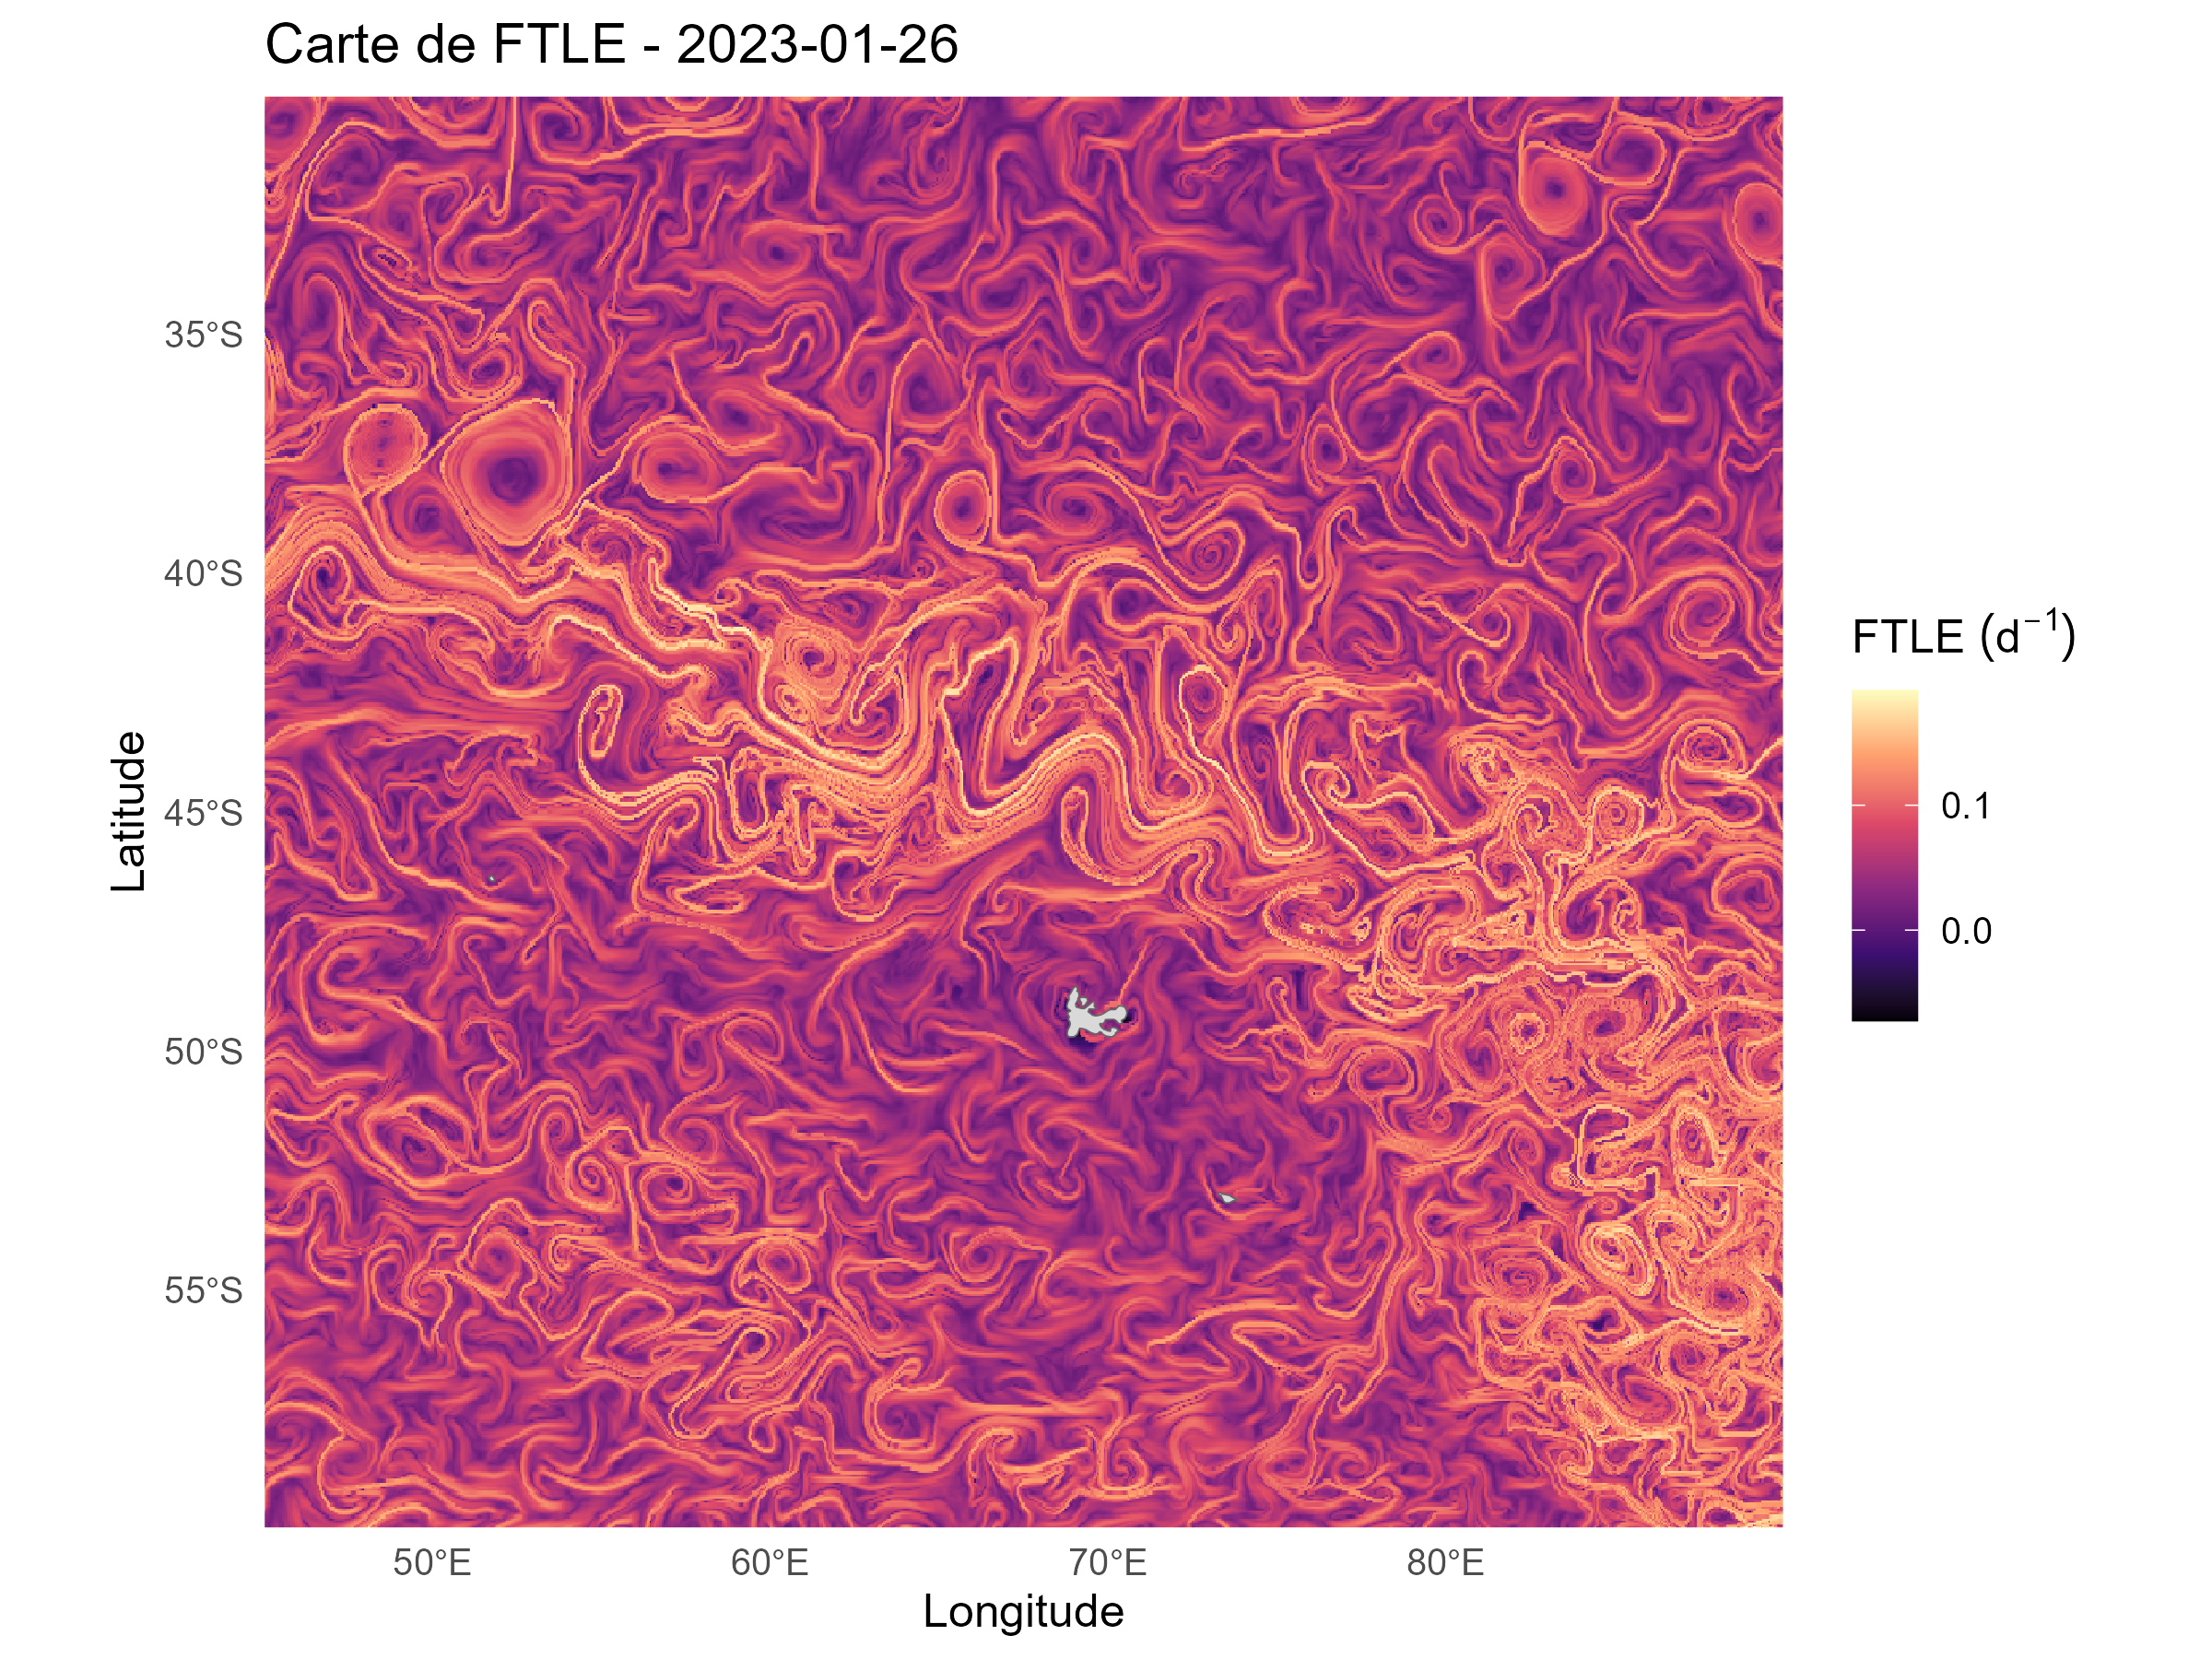
\includegraphics[width=0.5\textwidth]{images/02_materiel_et_methode/map_ftle_2023-01-26}
		\caption{Advection Lagrangienne FTLE backward (30j) du 2023-01-26. Les valeurs élevées de FTLE délimitent des crêtes correspondant à des frontières de transport de l'écoulement (de fronts ou de tourbillons) le long desquelles convergent les masses d'eau (structures cohérentes lagrangiennes attractives)}
		\label{fig:mapftle2023-01-26}
	\end{figure}
	 
	 Dans notre étude, la durée d'advection est de trente jours en backward, c'est-à-dire que les trajectoires sont intégrées vers l'arrière dans le temps (de $t$ à $t - T$). La résolution temporelle est journalière et la résolution spatiale est de 0.05°. La figure \ref{fig:mapftle2023-01-26} présente une carte de FTLE issue de la journée 2023-01-26. Les crêtes (valeur élevées) de FTLE marquent les zones où les particules voisines se séparent le plus fortement, ce qui permet d'identifier des structures physiques réelles de l'écoulement océanique.
	 
	 \subsection{Colocalisation des données par les plus proches voisins}